\documentclass[a4paper, 11pt]{article}
\usepackage{amsmath, amssymb}
\usepackage[margin=1in]{geometry}
\usepackage{graphicx}

\title{Machine Learning Homework Linear Classifiers}
\author{Vahid Maleki}
\date{\today}

\begin{document}
	\maketitle
	\section{Question One}
	Given:
	\[
	A^+ = \{(1, 1), (0, 2), (3, 0)\}, \quad A^- = \{(-2, -1), (0, -2)\}
	\]
	We augment the data points by adding a bias term of 1:
	\[
	A^+ = \{(1, 1, 1), (0, 2, 1), (3, 0, 1)\}, \quad A^- = \{(-2, -1, 1), (0, -2, 1)\}
	\]
	So our data points and labels is equal to
	\[
	\mathbf{X} = 
	\begin{bmatrix}
		1 & 1 & 1 \\
		0 & 2 & 1 \\
		3 & 0 & 1 \\
		-2 & -1 & 1 \\
		0 & -2 & 1
	\end{bmatrix}, \quad
	\mathbf{y} = 
	\begin{bmatrix}
		1 \\
		1 \\
		1 \\
		-1 \\
		-1
	\end{bmatrix}
	\]
	
	\section*{Solution to Part (a): Perceptron Learning Algorithm}
	
	Let the initial weight vector be:
	\[
	\mathbf{w}(0) = (0, 0, 0)
	\]
	The learning rate is $\eta = 1$. The Perceptron learning algorithm updates the weight vector for misclassified points.
	\\\\
	and the we check misclassification will the formula below:
	\[
	y_i w_i X_i \le 0
	\]
	
	\subsection*{Iteration 1}
	For the first point in $A^+$, $\mathbf{x}_1 = (1, 1, 1)$:
	\\\\
	check if \(y_i w_i X_i \le 0\):
	\[
	y_i (w_i X_i) = y_i (0\cdot1 + 0\cdot1 + 0\cdot1) = 0
	\]
	so we must update w
	\[
	\mathbf{w}(1) = \mathbf{w}(0) + \eta y_1 \mathbf{x}_1 = (0, 0, 0) + 1 \cdot 1 \cdot(1, 1, 1) = (1, 1, 1)
	\]
	
	\subsection*{Iteration 2}
	For the second point in $A^+$, $\mathbf{x}_2 = (0, 2, 1)$:
	\\\\
	check if \(y_i w_i X_i \le 0\):
	\[
	y_i (w_i X_i) = y_i (1\cdot0 + 1\cdot2 + 1\cdot1) = 3
	\]
	condition fails so we can't update w (there is not any misclassification)
	\\\\
	we can check all points but there is not any misclassification so after iteration 6 (iterating one time over data points) algorithm will stop.
	\\\\
	The final weight vector is:
	\[
	\mathbf{w}' = (1, 1, 1)
	\]
	To plot the separating line, we use the equation \( \mathbf{w} \cdot \mathbf{x} + b = 0 \). This is equivalent to:
	
	\[
	x_1 + x_2 + 1 = 0
	\]
	Thus, the equation of the separating line is:
	\[
	x_2 = -x_1 - 1
	\]
		
	\section*{Solution to Part (b): Least Squares Method}

	We aim to solve for $\mathbf{w}'$:
	\[
	 \mathbf{X}^T \mathbf{X} \mathbf{w}' =\mathbf{X}^T \mathbf{y}
	\]
	Where
	\[
	\mathbf{X} = 
	\begin{bmatrix}
		1 & 1 & 1 \\
		0 & 2 & 1 \\
		3 & 0 & 1 \\
		-2 & -1 & 1 \\
		0 & -2 & 1
	\end{bmatrix}, \quad
	\mathbf{y} = 
	\begin{bmatrix}
		1 \\
		1 \\
		1 \\
		-1 \\
		-1
	\end{bmatrix}
	\]
	We start with computing $\mathbf{X}^T \mathbf{X}$
	\[
	\mathbf{X}^T \mathbf{X} =
	\begin{bmatrix}
		1 & 0 & 3 & -2 & 0 \\
		1 & 2 & 0 & -1 & -2 \\
		1 & 1 & 1 & 1 & 1
	\end{bmatrix}
	\begin{bmatrix}
		1 & 1 & 1 \\
		0 & 2 & 1 \\
		3 & 0 & 1 \\
		-2 & -1 & 1 \\
		0 & -2 & 1
	\end{bmatrix}
	=
	\begin{bmatrix}
		14 & 3 & 2 \\
		3 & 10 & 0 \\
		2 & 0 & 5
	\end{bmatrix}
	\]
	then we should compute $\mathbf{X}^T \mathbf{y}$
	\[
	\mathbf{X}^T \mathbf{y} =
	\begin{bmatrix}
		1 & 0 & 3 & -2 & 0 \\
		1 & 2 & 0 & -1 & -2 \\
		1 & 1 & 1 & 1 & 1
	\end{bmatrix}
	\begin{bmatrix}
		1 \\
		1 \\
		1 \\
		-1 \\
		-1
	\end{bmatrix}
	=
	\begin{bmatrix}
		6 \\
		6 \\
		1
	\end{bmatrix}
	\]
	Finally we Solve for $\mathbf{w}'$
	\[
	\mathbf{w}' = (\mathbf{X}^T \mathbf{X})^{-1} \mathbf{X}^T \mathbf{y}
	\]
	we must make this matrix identity matrix:
	\[
	\begin{bmatrix}
		14 & 3 & 2 & | & 6\\
		3 & 10 & 0 & | & 6\\
		2 & 0 & 5 & | & 1
	\end{bmatrix}
	\]
	and after doing we end up with this matrix:
	\[
	\begin{bmatrix}
		1 & 0 & 0 & | & 0.31\\
		0 & 1 & 0 & | & 0.51\\
		0 & 0 & 1 & | & 0.07
	\end{bmatrix}
	\]
	To plot the separating line, we use the equation \( \mathbf{w} \cdot \mathbf{x} + b = 0 \). This is equivalent to:
	
	\[
	0.31 x_1 + 0.51 x_2 + 0.07 = 0
	\]
	Thus, the equation of the separating line is:
	
	\[
	x_2 = \frac{-0.31 x_1 - 0.07}{0.51}
	\]
	
	\section*{Solution to Part (c): Fisher Method:}
	
	fisrt we start by finding mean of \(A^+\) and \(A^-\) for each column
	\[
	\mathbf{\mu}_+ = \frac{1}{3} \sum_{x \in A^+} \mathbf{x} = \frac{1}{3} \left( (1,1) + (0,2) + (3,0) \right) = (1.33, 1)
	\]
	\[
	\mathbf{\mu}_- = \frac{1}{2} \sum_{x \in A^-} \mathbf{x} = \frac{1}{2} \left( (-2,-1) + (0,-2) \right) = (-1, -1.5)
	\]
	
	\subsection*{Compute the scatter matrices:}
	
	The \textbf{within-class scatter matrix} \( S_W \) is the sum of the scatter matrices of each class:
	\[
	S_W = S_+ + S_-
	\]
	Where \( S_+ \) and \( S_- \) are the within-class scatter matrices for \( A^+ \) and \( A^- \), respectively.
	\\\\
	For each point in class \( A^+ \), we compute:
	\[
	S_+ = \sum_{x \in A^+} (\mathbf{x} - \mathbf{\mu}_+)(\mathbf{x} - \mathbf{\mu}_+)^T
	\]
	Now we subtract the mean from each column
	\[
	(\mathbf{x} - \mathbf{\mu}_+) =
	\begin{pmatrix} 
		(1-1.33) & (1-1) \\ 
		(0-1.33) & (2-1) \\
		(3-1.33) & (0-1)
	 \end{pmatrix}
	\]
	And we multiply above matrix with it's transpose
	\[
	S_+ =
	\begin{pmatrix} 
		5.1 & -3.1 \\ 
		-3.1 & 2 \\
	\end{pmatrix}
	\]
	Similarly, for class \( A^- \):
	\[
	S_- = \sum_{x \in A^-} (\mathbf{x} - \mathbf{\mu}_-)(\mathbf{x} - \mathbf{\mu}_-)^T
	\]
	Now we subtract the mean from each column
	\[
	(\mathbf{x} - \mathbf{\mu}_-) =  
	\begin{pmatrix} 
		-2+1 & -1+1.5 \\
		0+1 & -2+1.5
	\end{pmatrix}
	\]
	And we multiply above matrix with it's transpose
	\[
	S_- = 
	\begin{pmatrix} 
		2 & -1 \\
		-1 & 0.5
	\end{pmatrix}
	\]
	Finally we add \(S_+\) and \(S_+\)
	\[
	S_W =  
	\begin{pmatrix} 
		5.01 & -3.1 \\
		-3.1 & 2
	\end{pmatrix}
	+
	\begin{pmatrix} 
		2 & -1 \\
		-1 & 0.5
	\end{pmatrix}
	=
	\begin{pmatrix} 
		7.1 & -4.1 \\
		-4.1 & 2.5
	\end{pmatrix}
	\]
	\subsection*{Compute the weights and bias:}
	We must compute the inverse of \(S_w\) and multiply it with differance of means
	\[
	w = S^{-1}_w(\mu^+ - \mu^-)
	\]
	
	\[
	w =  
	\begin{pmatrix} 
		3.5 & 5.75 \\
		5.75 & 9.8
	\end{pmatrix}
	\begin{pmatrix} 
		2.33 \\
		2.5
	\end{pmatrix}
	=
	\begin{pmatrix} 
		22.53 \\
		37.9
	\end{pmatrix}
	\]
	And $\mathbf{b}$ (intercept) can calculate with formula below
	\[
	b = - w^T \cdot \frac{(\mu^+ + \mu^-)}{2}
	\]
	\[
	b =
	\begin{pmatrix} 
		-22.53 & -37.9
	\end{pmatrix}
	\begin{pmatrix} 
		0.165 \\ 
		-0.25
	\end{pmatrix}
	= 5.76
	\]
	So the formula of line is 
	\[
	22.53 x_1 + 37.9 x_2 + 5.76 = 0
	\]
	\begin{figure}[h!]
		\centering
		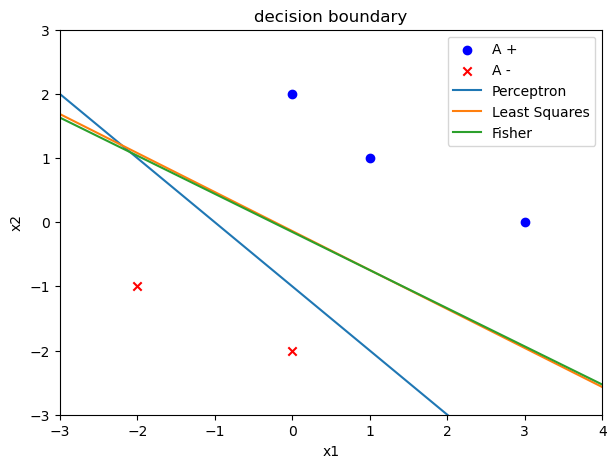
\includegraphics[width=0.65\textwidth]{images/q1.png}
		\caption{Decision Boundary}
		\label{fig:decision-boundary}
	\end{figure}
	
	\newpage
	\section{Question Two}
	
	Given two sets of points \( \{x_n\} \) and \( \{y_n\} \), their convex hulls are defined by:
	\[
	x = \sum_n \alpha_n x_n, \quad y = \sum_m \beta_m y_m,
	\]
	where \( \alpha_n, \beta_m \geq 0 \) and \( \sum_n \alpha_n = \sum_m \beta_m = 1 \).
	\\\\
	The sets \( \{x_n\} \) and \( \{y_n\} \) are linearly separable if there exists \( w \) and \( w_0 \) such that:
	\[
	w^T x_n + w_0 > 0 \quad \forall x_n, \quad w^T y_n + w_0 < 0 \quad \forall y_n.
	\]
	
	\subsection*{1. If Convex Hulls Intersect:} 
	
	If the convex hulls of \( \{x_n\} \) and \( \{y_n\} \) intersect, there exists a point \( z \) in both, which implies \( w^T z + w_0 > 0 \) and \( w^T z + w_0 < 0 \), a contradiction. Hence, they cannot be linearly separable.
	
	\subsection*{2. If Linearly Separable:} If a separating hyperplane exists, then \( w^T x + w_0 > 0 \) for all \( x \) in the convex hull of \( \{x_n\} \) and \( w^T y + w_0 < 0 \) for all \( y \) in the convex hull of \( \{y_n\} \). Thus, the convex hulls do not intersect.
	\\\\
	So if the convex hulls intersect, the sets are not linearly separable, and if they are linearly separable, their convex hulls do not intersect.
	
	\newpage
	\section{Question Three}
	
	\subsection*{(a) SGD Update Rule When \(\lambda = 0\)}
	
	When \(\lambda = 0\), the objective function reduces to just the logistic loss. The SGD update rule for \(w_i\) with step size \(\eta\) for the given example \((\mathbf{x}^{(j)}, y^{(j)})\) is:
	\[
	w_i \leftarrow w_i + \eta \cdot \left( y^{(j)} - \sigma\left( \sum_{k=1}^d w_k x_k^{(j)} \right) \right) x_i^{(j)}
	\]
	where \(\sigma(z) = \frac{1}{1 + e^{-z}}\) is the sigmoid function.
	
	\subsection*{(b) SGD Update Rule When \(\lambda > 0\)}
	
	When \(\lambda > 0\), the objective function includes the regularization term. The gradient of the regularization term with respect to \(w_i\) is:
	\[
	\frac{\partial}{\partial w_i} \left( -\frac{\lambda}{2} \sum_{k=1}^d w_k^2 \right) = -\lambda w_i
	\]
	\\
	Thus, the total gradient for \(w_i\) becomes:
	\[
	\frac{\partial F}{\partial w_i} = \left( y^{(j)} - \sigma\left( \sum_{k=1}^d w_k x_k^{(j)} \right) \right) x_i^{(j)} - \lambda w_i
	\]
	\\
	The SGD update rule for \(w_i\) is:
	\[
	w_i \leftarrow w_i + \eta \cdot \left[ \left( y^{(j)} - \sigma\left( \sum_{k=1}^d w_k x_k^{(j)} \right) \right) x_i^{(j)} - \lambda w_i \right]
	\]
	
	\subsection*{(c) Time Complexity Analysis}
	
	\textbf{Dense Data Structure:} \\
	In a dense representation, all \(d\) features are processed, including zeros. The average time complexity to update \(w_i\) is:
	\[
	O(d)
	\]
	\\
	\textbf{Sparse Data Structure:} \\
	In a sparse representation, only the non-zero elements of \(\mathbf{x}^{(j)}\) are processed. If \(s\) is the average number of non-zero features, the average time complexity to update \(w_i\) is:
	\[
	O(s)
	\]
	\\
	Since \(s \ll d\), using a sparse data structure significantly reduces computation time.
	
	\newpage
	\section{Question Four}
	\subsection*{Part (a): Classification of Classes 0 and 1}
	
	This section addresses the binary classification problem for classes 0 and 1 from the dataset. Three classifiers are implemented: Fisher's Linear Discriminant, Perceptron, and Least Squares. We discuss the implementation of each classifier, their decision boundaries, and compare their accuracy.
	
	\subsubsection*{1. Fisher's Linear Discriminant}
	
	To classify between classes 0 and 1, we start with Fisher’s Linear Discriminant, which aims to find a line that maximizes the separation between the two classes by projecting data points onto a single direction.
	The core code for calculating Fisher’s Linear Discriminant is:
	
	\begin{verbatim}
		mean_0 = np.mean(class_0, axis=0)
		mean_1 = np.mean(class_1, axis=0)
		S_0 = np.dot((class_0 - mean_0).T, (class_0 - mean_0))
		S_1 = np.dot((class_1 - mean_1).T, (class_1 - mean_1))
		S_w = S_0 + S_1
		w = np.linalg.inv(S_w).dot(mean_1 - mean_0)
		b = -np.dot(w, (mean_0 + mean_1) / 2)
	\end{verbatim}
	
	Here, \( \mathbf{w} \) is the weight vector that defines the direction of projection, and \( b \) is the bias term for the decision boundary. The samples are classified based on whether their projection along \( \mathbf{w} \) exceeds a threshold. The accuracy of Fisher’s classifier is calculated by comparing its predictions with the true labels.
	
	\subsubsection*{2. Perceptron}
	
	The Perceptron algorithm finds a linear boundary by iteratively adjusting weights based on classification errors. The main steps include initializing weights and bias, then updating these values based on misclassified samples.
	\\\\
	The core implementation for the Perceptron is:
	
	\begin{verbatim}
		w = np.zeros(X.shape[1])
		b = 0
		for i in range(len(y)):
			if y[i] * (np.dot(X[i], w) + b) <= 0:
				w += lr * y[i] * X[i]
				b += lr * y[i]
	\end{verbatim}
	
	In each iteration, if a sample is misclassified, the weight \( \mathbf{w} \) and bias \( b \) are updated. This process repeats for a fixed number of epochs. A threshold is then used for final classification, and the Perceptron’s accuracy is calculated.
	
	\subsubsection*{3. Least Squares Method}
	
	The Least Squares method solves the classification problem by minimizing the squared error. This is achieved by setting up the feature matrix \( \mathbf{X}_{\text{bias}} \) (with an additional bias term) and finding the weight vector \( \mathbf{w} \) that minimizes the mean squared error:
	
	\begin{verbatim}
		X_bias = np.c_[X, np.ones(X.shape[0])]
		wb = np.linalg.pinv(X_bias).dot(y)
		w, b = wb[:-1], wb[-1]
	\end{verbatim}
	
	Using the pseudoinverse \( \mathbf{X}_{\text{bias}}^+ \), we obtain both the weight vector \( \mathbf{w} \) and the bias term \( b \). This method provides a closed-form solution for linear classification, and its accuracy is computed by evaluating the predictions against the true labels.
	
	\subsubsection*{4. Accuracy Comparison and Results}
	
	Because the two class are completely separable all three algorithm do it perfectly:
	
	\begin{table}[h!]
		\centering
		\begin{tabular}{|c|c|}
			\hline
			\textbf{Classifier} & \textbf{Accuracy} \\
			\hline
			Fisher & 1.0 \\
			Perceptron & 1.0 \\
			Least Squares & 1.0 \\
			\hline
		\end{tabular}
		\caption{Accuracy Comparison of Fisher, Perceptron, and Least Squares Classifiers}
	\end{table}
	
	\subsubsection*{5. Decision Boundary Visualization}
	
	As you can see all three line separates the data perfectly and their weight and bias
	are very close to each other
	
	\begin{figure}[h!]
		\centering
		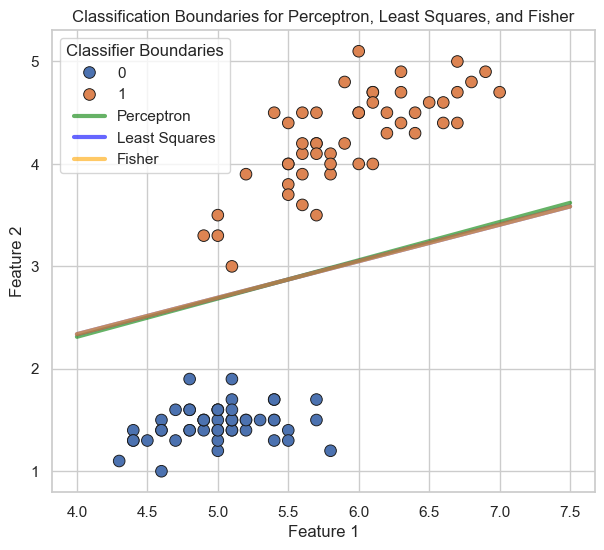
\includegraphics[width=0.6\textwidth]{images/q4_a.png}
		\caption{Classification Boundaries for Perceptron, Least Squares, and Fisher}
		\label{fig:decision_boundary}
	\end{figure}
	
	\newpage
	\subsection*{Part (b): Classification of Classes 1 and 2}
	
	In Part (b), we applied the same classification methods—Fisher’s Linear Discriminant, Perceptron, and Least Squares—on a binary classification problem involving only classes 1 and 2. The original labels were relabeled as follows for binary classification:
	\begin{itemize}
		\item Class 1 relabeled as 0.
		\item Class 2 relabeled as 1.
	\end{itemize}
	
	\subsubsection*{1. Data Preparation}
	
	The dataset was filtered to include only classes 1 and 2, after which the labels were updated to binary values to enable classification.
	
	\subsection*{2. Accuracy Comparison}
	
	The table below summarizes the accuracy of each classifier when applied to classes 1 and 2:
	
	\begin{table}[h!]
		\centering
		\begin{tabular}{|c|c|}
			\hline
			\textbf{Classifier} & \textbf{Accuracy} \\
			\hline
			Fisher (Classes 1 \& 2) & 0.94 \\ 
			Perceptron (Classes 1 \& 2) & 0.93 \\ 
			Least Squares (Classes 1 \& 2) & 0.94 \\ 
			\hline
		\end{tabular}
		\caption{Accuracy Comparison of Fisher, Perceptron, and Least Squares Classifiers for Classes 1 and 2}
	\end{table}
	
	\subsection*{3. Decision Boundary Visualization}
	
	As you can see in Figure~\ref{fig:decision_boundary_b} Classification Boundaries for Fisher and Least Squares are very similar and perceptron is a bit differant.
	
	\begin{figure}[h!]
		\centering
		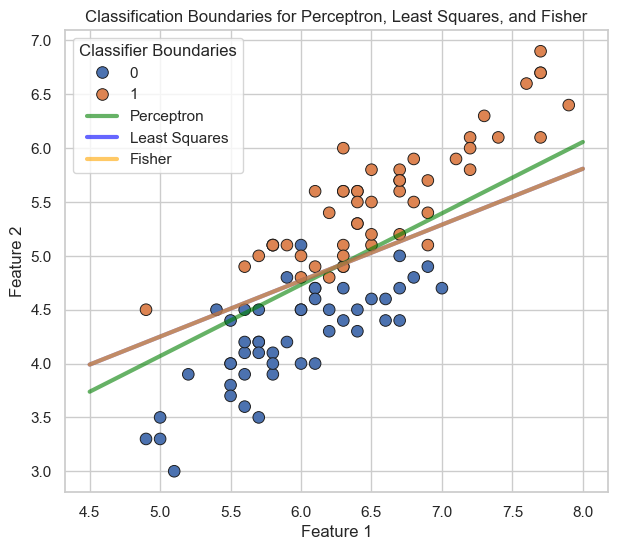
\includegraphics[width=0.6\textwidth]{images/q4_b.png}
		\caption{Classification Boundaries for Perceptron, Least Squares, and Fisher (Classes 1 and 2)}
		\label{fig:decision_boundary_b}
	\end{figure}
	
	\subsection*{Part (c): Analysis of Results from Parts (a) and (b)}
	
	In this section, we compare the performance of the classifiers between the tasks in Parts (a) and (b).
	
	\subsubsection*{Performance Differences Between Part (a) and Part (b)}
	
	\begin{itemize}
		\item \textbf{Classes 0 and 1 (Part (a))}: All three classifiers—Fisher’s Linear Discriminant, Perceptron, and Least Squares—performed reasonably well on classes 0 and 1. This suggests that classes 0 and 1 are \textit{more linearly separable} in the provided feature space, allowing each classifier to find an effective linear boundary.
		\item \textbf{Classes 1 and 2 (Part (b))}: The Perceptron struggled with classification on classes 1 and 2, indicating that these classes are \textit{less linearly separable} or have a significant degree of overlap. Fisher’s Linear Discriminant and the Least Squares method handled the overlap better, achieving reasonable accuracy but with a slight drop compared to Part (a).
	\end{itemize}
	
	\subsection*{Conclusion}
	
	\begin{itemize}
		\item \textbf{Linearly Separable vs. Non-Linearly Separable Classes}: The classifiers performed better on linearly separable classes (Part (a)). The overlap between classes in Part (b) made classification more challenging, especially for the Perceptron.
		\item \textbf{Fisher’s and Least Squares Robustness}: Fisher’s Linear Discriminant and the Least Squares method showed robustness to overlapping classes, as they could handle non-perfect separability better than the Perceptron.
	\end{itemize}
	
	\newpage
	\subsection*{Part (d): Logistic Regression for Classes 0 \& 1 and Classes 1 \& 2}
	
	In Part (d), we applied Logistic Regression to the same binary classification tasks as in Parts (a) and (b) to compare its performance with the previously tested classifiers.
	
	\subsection*{Results}
	
	The accuracies of Logistic Regression on classes 0 \& 1 (Part (a)) and classes 1 \& 2 (Part (b)) are similar to the algorithms that we have already implemented.
	
	\begin{table}[h!]
		\centering
		\begin{tabular}{|c|c|}
			\hline
			\textbf{Classifier} & \textbf{Accuracy} \\
			\hline
			Logistic Regression (Classes 0 \& 1) & 1.0 \\ 
			Logistic Regression (Classes 1 \& 2) & 0.94 \\ 
			\hline
		\end{tabular}
		\caption{Logistic Regression accuracy for binary classification tasks.}
	\end{table}
	
	
	
	\newpage
	\subsection*{Part (e): Multiclass Classification Using Least Squares}
	
	In Part (e), we extended the classification task to a multiclass problem involving all three classes (0, 1, and 2) using a one-vs-all approach with Least Squares.
	
	\subsection*{Methodology}
	
	\begin{itemize}
		\item \textbf{One-hot Encoding}: We one-hot encoded the target labels to handle the multiclass classification as a regression problem using the Least Squares method.
		\item \textbf{Bias Term}: A bias term was added by augmenting the feature matrix with a column of ones.
		\item \textbf{Weights Calculation}: The weights were computed using the normal equation: \[ W = (X^T X)^{-1} X^T Y \] where \( Y \) is the one-hot encoded target matrix.
	\end{itemize}
	
	\subsection*{Results}
	
	The accuracy of the multiclass Least Squares classifier on the entire dataset was as follows:
	
	\begin{itemize}
		\item \textbf{Accuracy}: 0.7933
	\end{itemize}
	
	This accuracy reflects the classifier’s ability to handle all three classes in a single model, though it may still be affected by overlapping classes.
	
	\end{document}
	
	
\end{document}
